\documentclass[11pt]{article}

\usepackage[margin=1in]{geometry}
\usepackage{graphicx}
\usepackage{booktabs}
\usepackage{array}
\usepackage{xcolor}
\usepackage{amsmath}
\usepackage{amssymb}
\usepackage{caption}
\usepackage{float}
% placeins unavailable on this system; with [H] floats are placed in-line, so
% a no-op \FloatBarrier suffices to keep each figure with its paragraph.
\providecommand{\FloatBarrier}{}
\usepackage[colorlinks=true,linkcolor=accent,urlcolor=accent,citecolor=accent]{hyperref}

% --- both figure roots: our solo PNGs + composites, and the raw paper crops ---
\graphicspath{{figures_solo/}{../../references/paper_figures/}}

% --- colours ---
\definecolor{accent}{RGB}{20,90,150}
\definecolor{accentlight}{RGB}{232,240,248}
\definecolor{warn}{RGB}{150,70,20}
\definecolor{warnlight}{RGB}{250,240,228}
\definecolor{rulegray}{RGB}{120,120,120}

% --- section heading styling: a touch of colour + a rule ---
\makeatletter
\renewcommand\section{\@startsection{section}{1}{\z@}%
  {-3.5ex \@plus -1ex \@minus -.2ex}%
  {2.3ex \@plus.2ex}%
  {\normalfont\Large\bfseries\color{accent}}}
\renewcommand\subsection{\@startsection{subsection}{2}{\z@}%
  {-3.25ex\@plus -1ex \@minus -.2ex}%
  {1.5ex \@plus .2ex}%
  {\normalfont\large\bfseries\color{accent}}}
\makeatother

\captionsetup{font=small,labelfont={bf,color=accent}}
\setlength{\parskip}{0.4em}
\setlength{\parindent}{0pt}

% --- headline / callout boxes: framed minipage fallback ---
\newcommand{\headlinebox}[1]{%
  \begin{center}
  \setlength{\fboxsep}{12pt}%
  \setlength{\fboxrule}{1.2pt}%
  \fcolorbox{accent}{accentlight}{%
    \begin{minipage}{0.92\textwidth}
    #1
    \end{minipage}}%
  \end{center}}
\newcommand{\warnbox}[1]{%
  \begin{center}
  \setlength{\fboxsep}{12pt}%
  \setlength{\fboxrule}{1.2pt}%
  \fcolorbox{warn}{warnlight}{%
    \begin{minipage}{0.92\textwidth}
    #1
    \end{minipage}}%
  \end{center}}

\begin{document}

% ===================== TITLE BLOCK =====================
\begin{center}
{\color{accent}\rule{\textwidth}{1.5pt}}\\[1.2em]
{\LARGE\bfseries Paper vs.\ Ours, with Custodial:\\[0.3em]
A Constraint-by-Constraint Comparison\par}
\vspace{0.8em}
{\large How custodial symmetry changes (and does not change)\\
each RS flavor / electroweak constraint we run.\par}
\vspace{0.7em}
{\large June 2026\par}
\vspace{0.4em}
{\color{accent}\rule{\textwidth}{1.5pt}}
\end{center}
\vspace{1em}

% ===================== INTRODUCTION =====================
\section{Introduction}

This note answers one question: \textbf{how does custodial symmetry
($\mathrm{SU(2)}_L\times\mathrm{SU(2)}_R\times\mathrm{U(1)}_X\times P_{LR}$)
affect the constraints we actually run in our minimal-RS scan?} For each
observable we put the \textbf{published figure on the left} and \textbf{our
fixed-code reproduction on the right}, focusing on what custodialization does to
the floor.

\textbf{The one-line answer.} Custodial symmetry is an \emph{electroweak} cure,
not a \emph{flavor} cure. It protects the oblique $T$ parameter and the
$Z\,b_L\bar b_L$ vertex, pulling the EW floors down from ${\sim}16$--$20$~TeV
(ours, minimal) to a few TeV. It does \textbf{nothing} to the $\varepsilon_K$
wall, which stays at tens of TeV --- because the binding kaon operator is the
color-octet KK-gluon $\mathrm{LR}/C_4$ operator, an electroweak singlet that the
custodial group cannot touch. This is not a feature of our proxy: Blanke et al.\
(0809.1073) computed the \emph{full} $\Delta F=2$ \emph{inside the custodial
model} and still found $M_{KK}\gtrsim18$--$30$~TeV from $\varepsilon_K$.

\textbf{Lane note.} The $\varepsilon_K$ comparisons here use our
\textbf{anarchic baseline (lane A)} --- the literature strawman --- so they line
up against Bauer / CFW / Blanke. Production as run (lane B, fit-aligned MFV) is a
sharper wall at $\approx$7~TeV, and the FPR/aligned ideal (lane C) is
$\approx$2~TeV. Custodial does not move \emph{any} of these flavor lanes; only
\emph{flavor alignment} does. Canonical lane definitions:
\texttt{docs/MODEL\_CONVENTIONS.md}.

% ===================== REAL vs PROXY CALLOUT =====================
\section{Real physics vs.\ proxy limitation}

Before the comparisons, one honest caveat. When our code shows custodial touching
\textbf{only} $S,T,U$ and $Z\to b\bar b$ and \emph{nothing} in flavor, that is
\textbf{${\sim}90\%$ real physics and ${\sim}10\%$ a proxy limitation}. The two
must not be conflated.

\warnbox{%
{\large\bfseries\color{warn} REAL (literature-confirmed) vs.\ PROXY (genuinely missing)}\\[0.6em]
\textbf{REAL --- the $\varepsilon_K$ wall is genuinely custodial-blind.}
$\varepsilon_K$ is dominated by the \textbf{KK-gluon} $\mathrm{LR}/C_4$ operator.
The KK gluon is a \emph{color octet, electroweak singlet} --- uncharged under the
custodial group, which is purely electroweak --- so custodialization
\emph{cannot} change the leading $\varepsilon_K$ amplitude. This is confirmed by a
\textbf{full calculation, not our proxy}: \textbf{Blanke 2008} (0809.1073)
computed the complete $\Delta F=2$ inside the custodial model (custodians, EW KK
bosons, everything) and still found $M_{KK}\gtrsim18$--$30$~TeV. Bauer~II
(0912.1625): $C_4$ ``is a pure QCD effect $\ldots$ insensitive to the precise
embedding of the electroweak gauge symmetry.''\\[0.5em]
\textbf{PROXY LIMITATION --- what we genuinely omit.} Our implementation is a
\textbf{leading-order tree EW proxy}, not the full custodial model. It does NOT
implement: the \emph{custodian KK-fermion spectrum} (charge-$5/3$ states,
bidoublet partners); the \emph{subleading custodial flavor effects} custodial
\emph{does} touch (EW KK bosons --- KK-$Z$, $Z'$, $Z_H$ --- contributing to
$\Delta F=2$; custodian loops in $b\to s\gamma$); the \emph{full} $\Delta T$
(singlet-only, dropping the dominant negative bidoublet $\Delta T$); a non-trivial
$b_R$ representation ($g_R^b$ is hard-zeroed).\\[0.5em]
\textbf{Therefore:} the headline \emph{``custodial fixes EW (${\sim}2$--$3$~TeV)
but not the $\varepsilon_K$ wall (tens of TeV)''} is REAL and
literature-confirmed. The stronger-sounding \emph{``custodial does literally
nothing to any flavor observable''} --- what our code prints --- is partly a
proxy limitation. \textbf{The plots below use the LEADING custodial physics only,
which we implement correctly.} This proxy is adequate for the RS-vs-SM note's
thesis; it is \emph{not} adequate for custodial phenomenology ($A_{FB}^b$,
$b\to s\gamma$, the subleading custodial $\Delta F=2$, the precise custodial EW
floor) --- that is the deferred full custodial build (roadmap D), scoped by the
four proxy items in \S\ref{sec:gaps}.
}

\FloatBarrier
\clearpage

% ===================== SIDE-BY-SIDE COMPARISONS =====================
\section{Side-by-side: paper vs.\ ours, constraint by constraint}

In every composite below the \textbf{\textcolor{warn}{PAPER}} panel (the cropped
published figure) is on the left and \textbf{\textcolor{accent}{OURS}} (our
fixed-code reproduction) is on the right.

% ---------------- (a) S,T,U ----------------
\subsection{(a)\quad $S,T,U$ oblique --- custodial protects $T$, not $S$}

\begin{figure}[H]
\centering
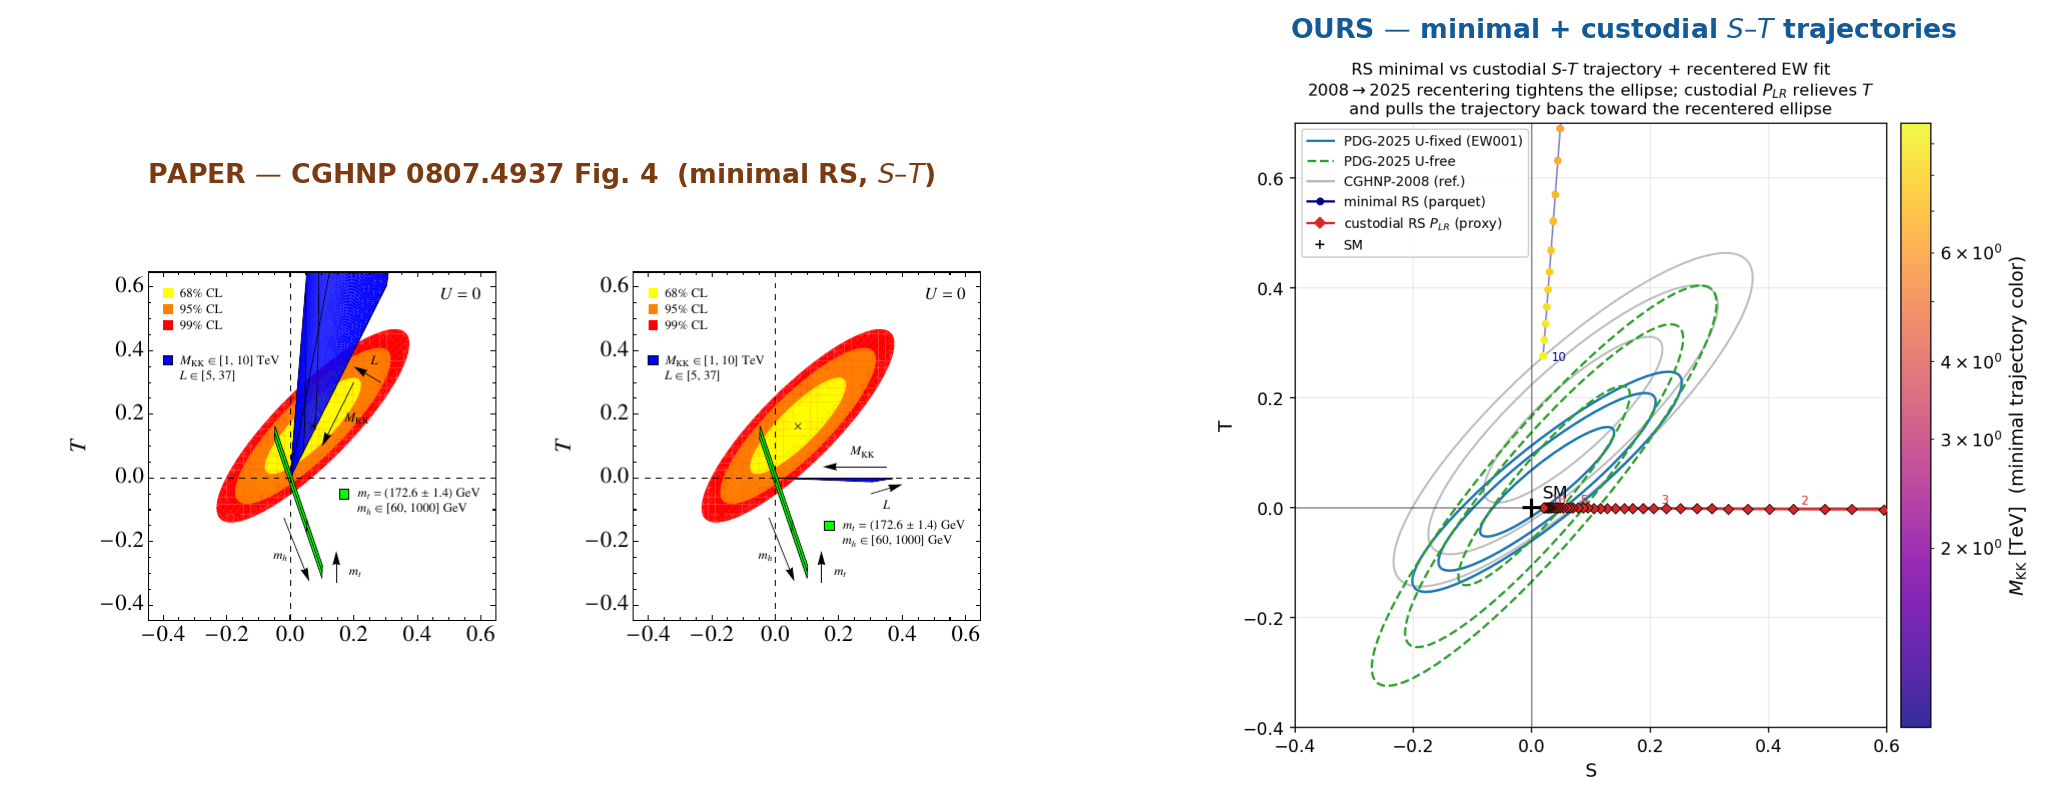
\includegraphics[width=\textwidth]{sxs_STU.png}
\caption{\textbf{Oblique $S$--$T$.} \emph{Left (paper):} CGHNP 0807.4937 Fig.~4,
minimal RS sweeping a wedge that climbs steeply in $T$ (the volume-enhanced ``RS
$T$ problem,'' $T\propto\pi L/(2\cos^2\theta_W)\cdot v^2/M_{KK}^2$). \emph{Right
(ours):} the same minimal trajectory (it shoots up in $T$) plus the
\textbf{custodial $P_{LR}$ trajectory}, which runs almost flat along the $S$-axis
($T\to0$) --- the ADMS mechanism (SU(2)$_R$ kills the $\log(L{\approx}30)$
enhancement, $\Delta T\propto+L\to-1/L$). Custodial relieves the irreducible
oblique floor: \textbf{our minimal ${\sim}16$--$20$~TeV $\to$ custodial
${\sim}6$~TeV}; the residual is set by the \emph{unprotected} $S$ (literature
custodial floor ${\sim}2.5$--$3$~TeV, $S$-limited). $S$ carries no symmetry
protection, so it sets the wall.}
\end{figure}

\FloatBarrier

% ---------------- (b) Z->bb ----------------
\subsection{(b)\quad $Z\to b\bar b$ --- $P_{LR}$ protects $g_L^b$ at tree, loops re-introduce it}

\begin{figure}[H]
\centering
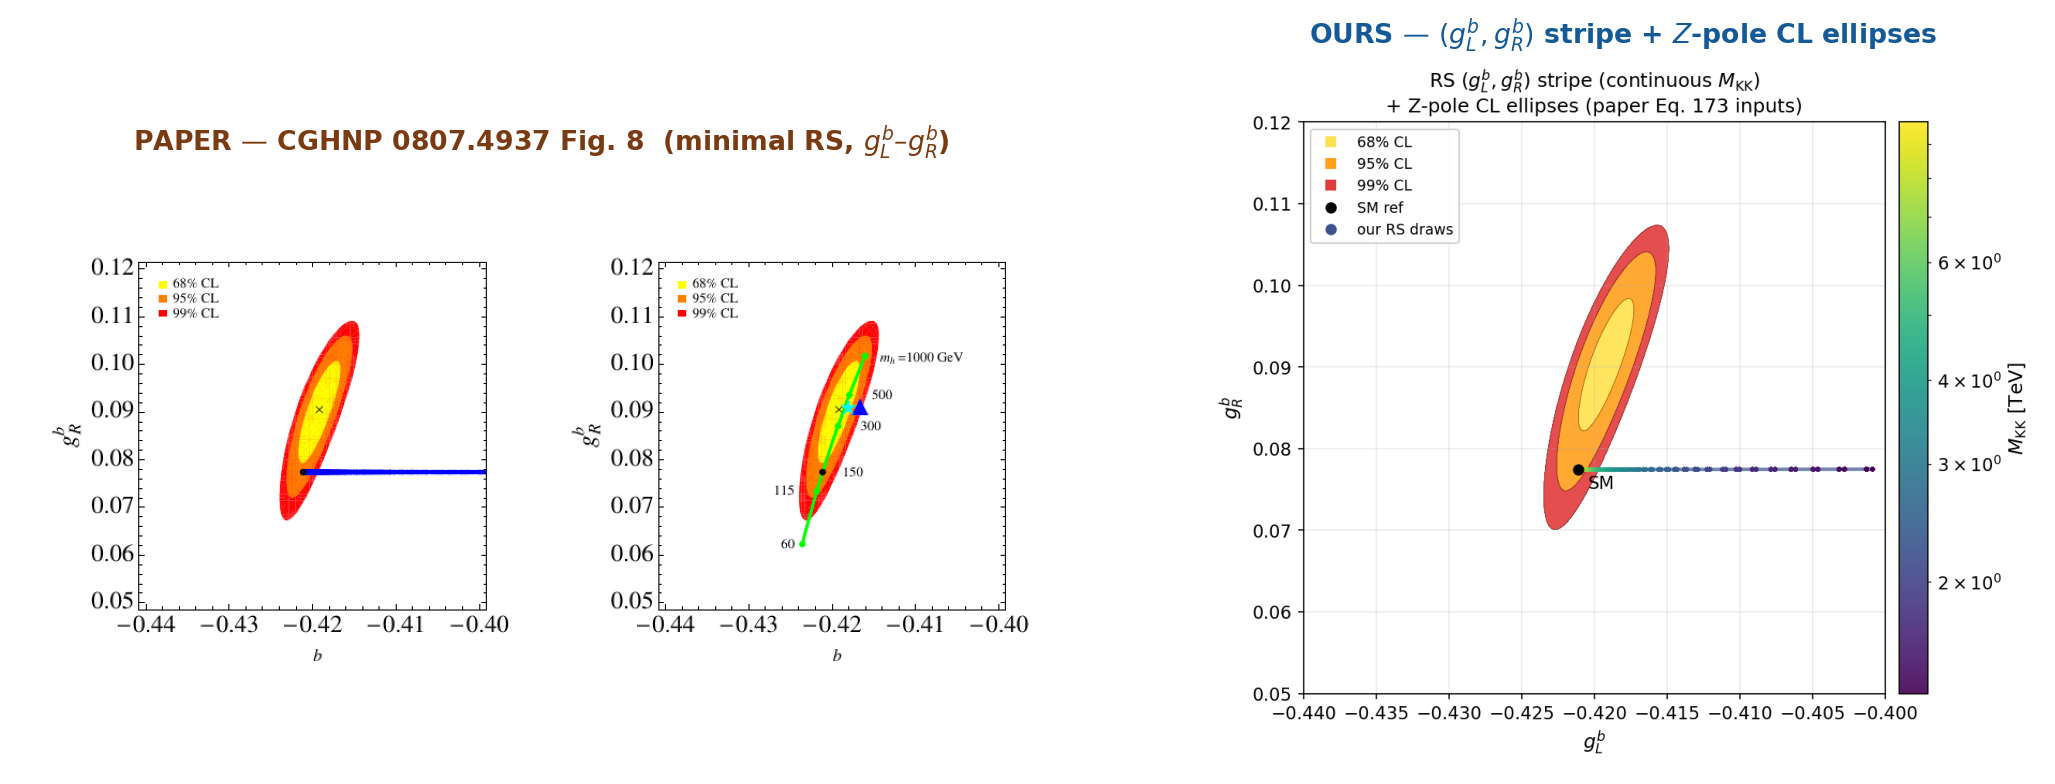
\includegraphics[width=\textwidth]{sxs_Zbb_top.png}
\caption{\textbf{$Z\to b\bar b$ couplings, minimal.} \emph{Left (paper):} CGHNP
0807.4937 Fig.~8, the $(g_L^b,g_R^b)$ plane with the $Z$-pole 68/95/99\% CL
ellipses and the minimal-RS scatter. \emph{Right (ours):} our $(g_L^b,g_R^b)$
stripe overlays the same ellipses and SM point (sanity check). With the B1 fix the
total coupling shift is gauge-KK dominated and moves $g_L^b$ to less-negative
values as $M_{KK}$ drops --- the CGHNP direction. In \emph{minimal} RS this bites
only to ${\sim}5$~TeV (the old $25$--$30$~TeV ``$Z\to b\bar b$ floor'' was a
sign-bug artifact).}
\end{figure}

\FloatBarrier

\begin{figure}[H]
\centering
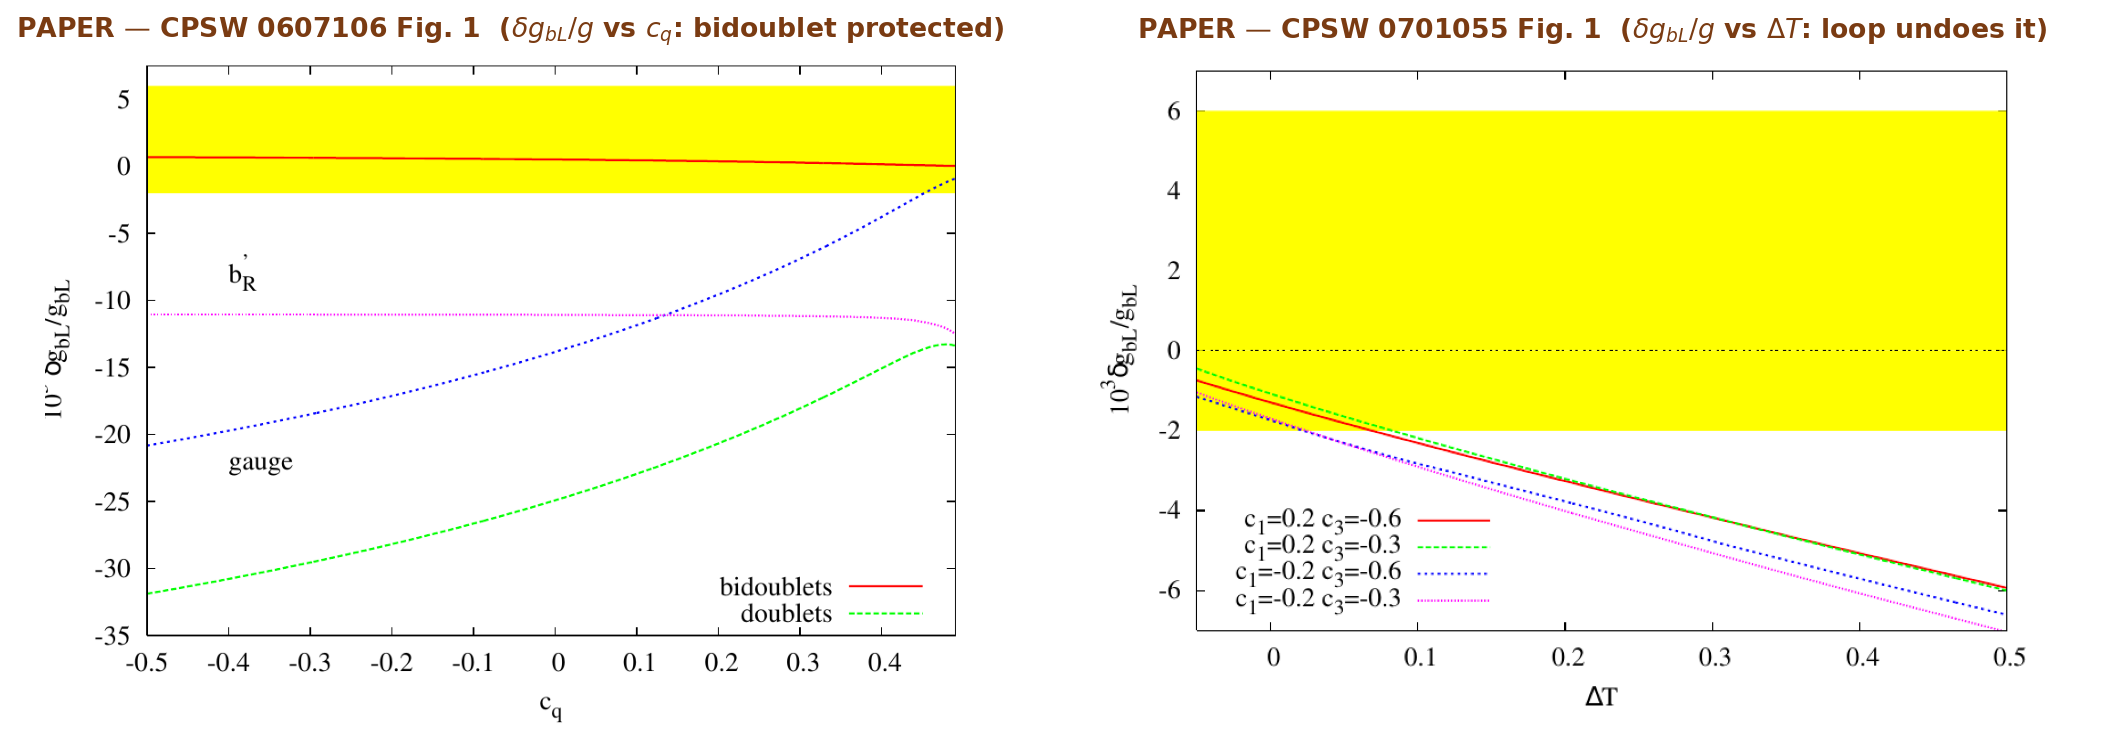
\includegraphics[width=\textwidth]{sxs_Zbb_cpsw.png}
\caption{\textbf{$Z\to b\bar b$ under custodial (CPSW).} \emph{Left:} CPSW
hep-ph/0607106 Fig.~1 --- $\delta g_{bL}/g$ vs.\ $c_q$. The \textbf{bidoublet}
embedding (red) sits inside the yellow allowed band: $P_{LR}$ with
$b_L\in(2,2)_{2/3}$ \textbf{zeroes $\delta g_L^b$ at tree level} (ACDP), whereas
the unprotected ``gauge''/``doublets'' curves run far below. \emph{Right:} CPSW
hep-ph/0701055 Fig.~1 --- $\delta g_{bL}/g$ vs.\ $\Delta T$. The top-partner
\textbf{one-loop} corrections \textbf{re-introduce} a negative $\delta g_L^b$,
correlated with $+\Delta T$; the curves exit the $2\sigma$ band by
$\Delta T\approx0.2$--$0.5$. So $P_{LR}$ (ACDP) zeroes $\delta g_L^b$ at tree, but
the top partners (CPSW) bring it back at loop --- the custodial $Z\to b\bar b$
story is a tree-protection that loops partially undo, which our loop proxy
reproduces (CPSW Eqs.~13--15).}
\end{figure}

\FloatBarrier
\clearpage

% ---------------- (c) eps_K ----------------
\subsection{(c)\quad $\varepsilon_K$ --- the wall does NOT move under custodial}

\begin{figure}[H]
\centering
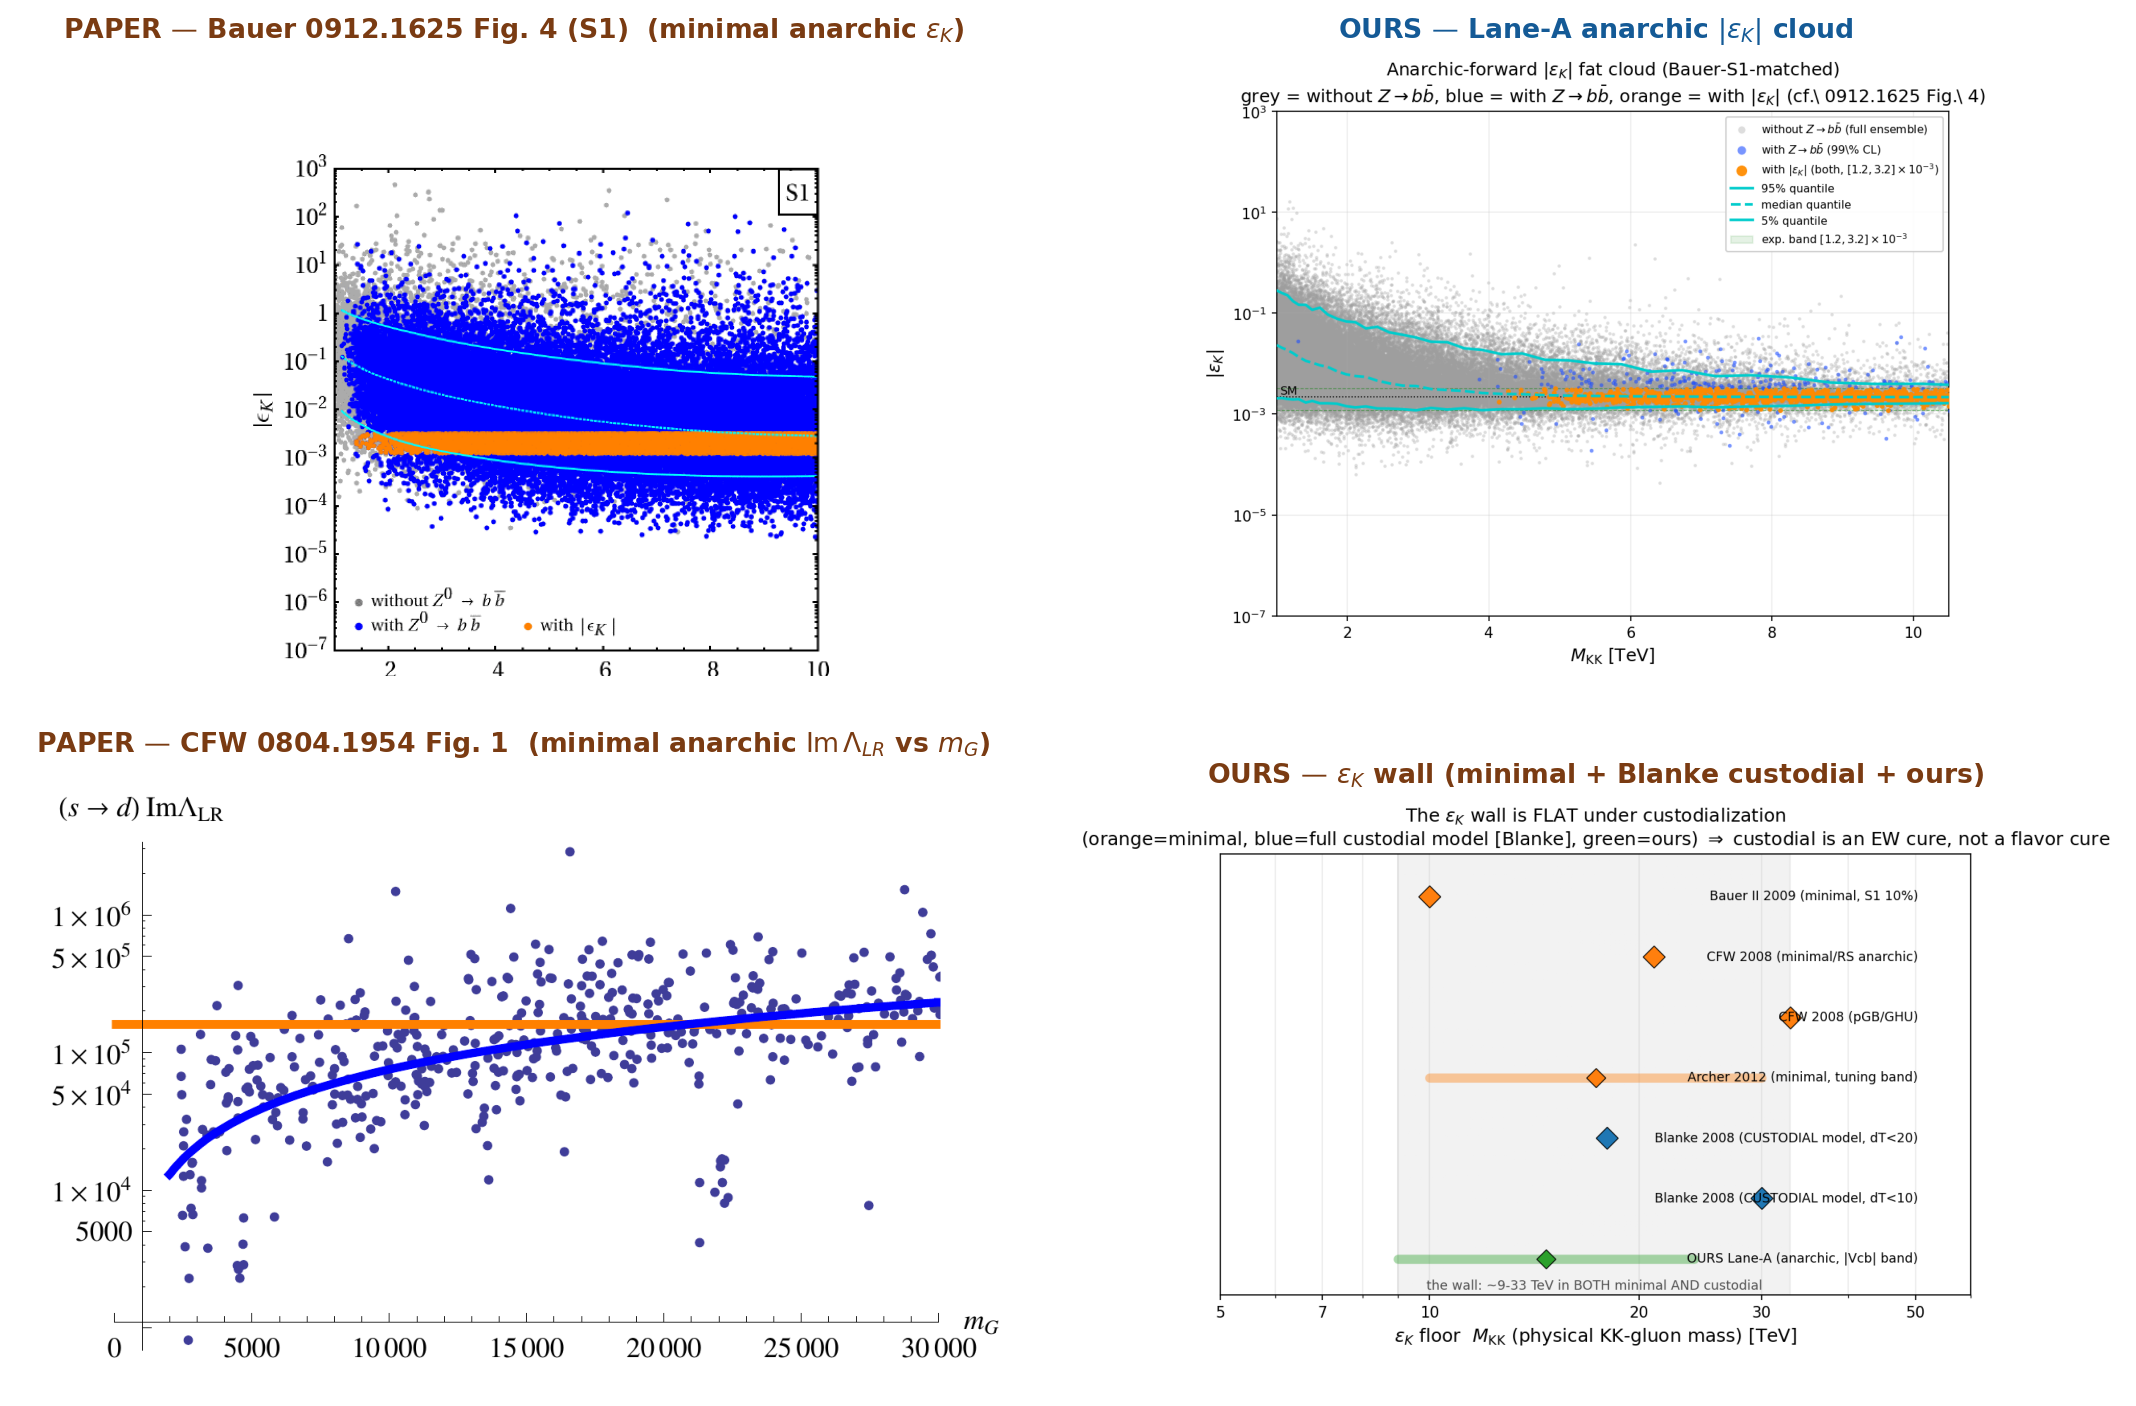
\includegraphics[width=\textwidth]{sxs_epsK_min.png}
\caption{\textbf{$\varepsilon_K$ --- the MINIMAL anarchic wall.}
\emph{Top-left (paper):} Bauer 0912.1625 Fig.~4 (S1), the anarchic
$|\varepsilon_K|$ cloud spanning ${\sim}6$ decades; the 95\%-quantile floor sits
at $M_g^{(1)}\gtrsim10$~TeV. \emph{Top-right (ours):} our Lane-A anarchic
$|\varepsilon_K|$ cloud (Bauer-S1-matched), same ${\sim}6$-decade spread, same
grey/blue/orange colouring and 5/50/95\% quantiles. \emph{Bottom-left (paper):}
CFW 0804.1954 Fig.~1, the anarchic $\mathrm{Im}\,\Lambda_{LR}$ ($s\to d$) KK-gluon
scan vs.\ $m_G$, crossing the bound (orange) around $m_G\approx20$~TeV.
\emph{Bottom-right (ours):} our $\varepsilon_K$ floor scoreboard --- minimal
literature anchors, the Blanke custodial anchors, and our Lane-A band, all in the
${\sim}9$--$33$~TeV wall. The point: in \emph{minimal} RS the wall is tens of TeV.}
\end{figure}

\FloatBarrier

\begin{figure}[H]
\centering
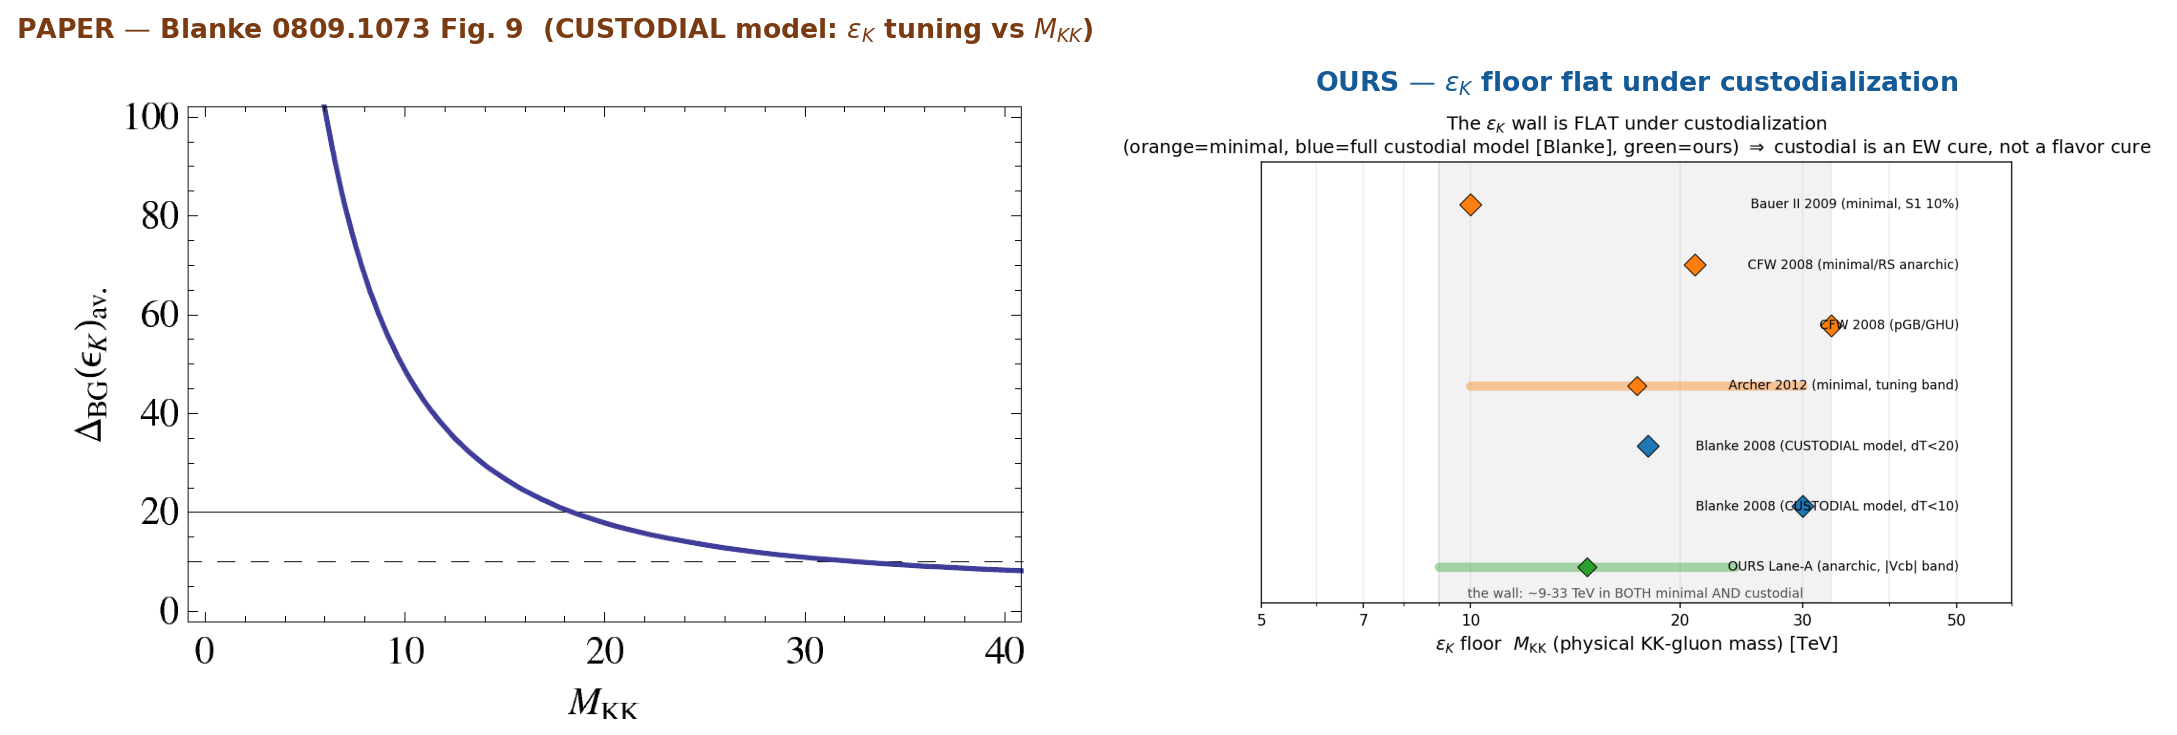
\includegraphics[width=\textwidth]{sxs_epsK_cust.png}
\caption{\textbf{$\varepsilon_K$ --- the CUSTODIAL model gives the SAME wall.}
\emph{Left (paper):} Blanke 0809.1073 Fig.~9 --- the $\varepsilon_K$ fine-tuning
$\Delta_{BG}(\varepsilon_K)$ vs.\ $M_{KK}$ computed \textbf{inside the full
custodial model}. The curve crosses $\Delta<20$ at $M_{KK}\approx18$~TeV and
$\Delta<10$ at $M_{KK}\approx30$~TeV --- the wall \textbf{survives
custodialization}. \emph{Right (ours):} our flat-wall scoreboard puts the Blanke
\emph{custodial} anchors (18/30~TeV) right on top of the \emph{minimal}
Bauer/CFW/Archer anchors and our Lane-A band. \textbf{The $\varepsilon_K$ wall
does not move under custodial} --- in the literature (Blanke's full calculation)
and in ours. This is the crux: custodial is an EW cure, not a flavor cure.}
\end{figure}

\FloatBarrier
\clearpage

% ---------------- (d) synthesis ladder ----------------
\subsection{(d)\quad Synthesis: the custodial decoupling ladder}

\begin{figure}[H]
\centering
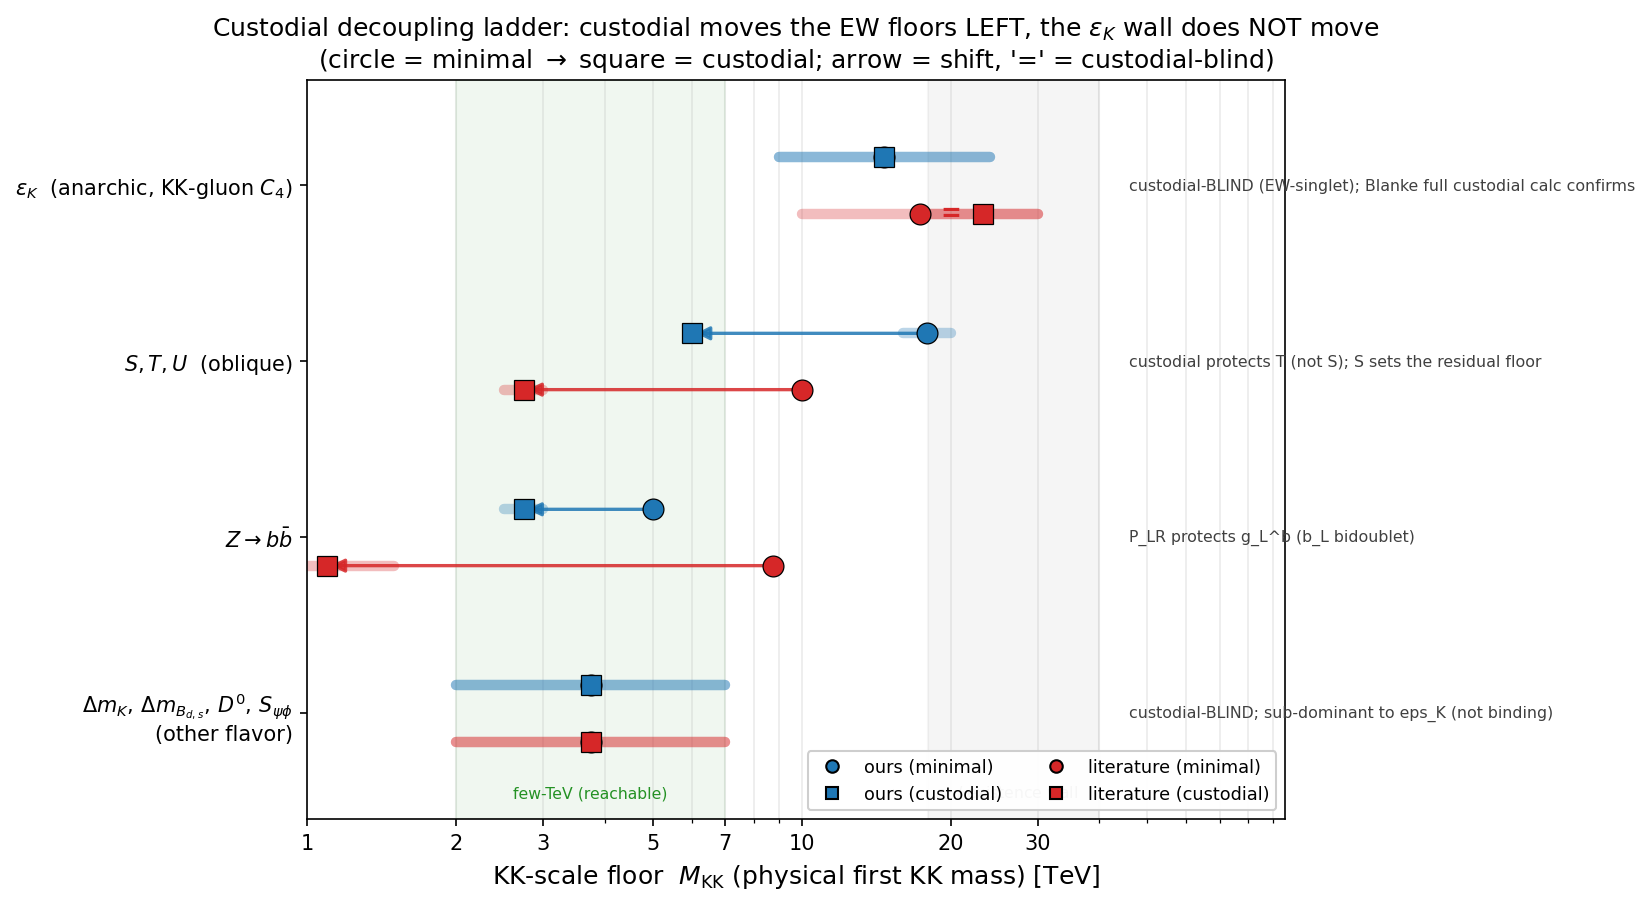
\includegraphics[width=\textwidth]{custodial_decoupling_ladder.png}
\caption{\textbf{The whole story on one axis.} Per-constraint KK-mass floor,
minimal (circle) $\to$ custodial (square), ours (blue) and literature (red). The
\textbf{electroweak} floors ($S,T,U$ and $Z\to b\bar b$) move \textbf{left} under
custodial (arrows); the \textbf{$\varepsilon_K$ wall and the other flavor
constraints do not move} (``$=$''). Custodial brings the EW sector into the
few-TeV reachable band (green) but leaves the $\varepsilon_K$/existence wall at
tens of TeV (grey).}
\end{figure}

\FloatBarrier
\clearpage

% ===================== TABLES =====================
\section{Provenance, attribution, and literature floors}

{\sloppy
These tables condense the three custodial provenance documents in
\texttt{docs/}: \texttt{CUSTODIAL\_PROVENANCE.md} (where every equation comes
from), \texttt{CUSTODIAL\_PLOTS\_AND\_ATTRIBUTION.md} (who computed what), and
\texttt{CUSTODIAL\_LITERATURE\_CATALOG.md} (per-paper floors). Status tags:
\textbf{S} = sourced (exact published equation),
\textbf{T} = faithful truncation (documented simplification),
\textbf{P} = proxy (correct parametric form, underived coefficients/inputs).
\par}

% ---- master provenance table ----
\subsection{Master provenance: where every custodial equation comes from}

\begin{center}
\footnotesize
\renewcommand{\arraystretch}{1.25}
\setlength{\tabcolsep}{4pt}
\begin{tabular}{@{}>{\raggedright\arraybackslash}p{0.255\textwidth}>{\raggedright\arraybackslash}p{0.205\textwidth}>{\raggedright\arraybackslash}p{0.145\textwidth}c>{\raggedright\arraybackslash}p{0.185\textwidth}@{}}
\toprule
\textbf{Code quantity} & \textbf{Form} & \textbf{Source} & \textbf{Tag} & \textbf{Gap?} \\
\midrule
minimal $\Delta T$ & $x_1^2\,\pi L/(2c_W^2)(v/M)^2$ & CGHNP (147) & T & leading-$L$ (0.04\% cons.) \\
custodial $\Delta T$ & $-x_1^2\,\pi/(4c_W^2 L)(v/M)^2$ & CGHNP (153) $\leftarrow$ ADMS & S & in-code cite missing \\
$\Delta S$ & $c_S(v/M)^2,\ c_S{=}30$ & PDG-2025 & S & --- \\
$\Delta U$ & $0$ & CGHNP/ADMS & S & --- \\
minimal $g_L^b$ & $+(m_b^2/2M^2)B_d$ & CGHNP (170) & S & convention caveat \\
minimal $g_R^b$ & $-(m_b^2/2M^2)B_Q$ & CGHNP (170) & S & convention caveat \\
custodial $g_L^b\to0$ & $P_{LR}$ zeroing & ACDP (3)--(12) & S & --- \\
custodial $g_L^b$ residual & $\kappa_b(1/L)g_L^{b,\min}$ & --- & \textbf{P} & \textbf{ad hoc knob} \\
custodial $g_R^b{=}0$ & $g_R^b\to0$ & ACDP (22)/Tab.\,1 & T & rep not pinned \\
loop $\delta g_L^b$ singlet & CPSW (14) & CPSW-ob (14) & S & --- \\
loop $\delta g_L^b$ bidoublet & CPSW (15) & CPSW-ob (15) & S & --- \\
loop $\Delta T$ singlet & CPSW (13)+(35) & CPSW (13)/(43) & T & drops neg.\ bidoublet $\Delta T$ \\
loop $\delta g_R^b{=}0$ & $0$ & CPSW-ob (p.10) & S & --- \\
loop inputs $\xi,\rho$ & $M_t{=}\rho_t M,\dots$ & --- & \textbf{P} & \textbf{breaks wavefn.\ corr.} \\
\bottomrule
\end{tabular}
\end{center}

Bottom line: \emph{every closed-form equation} in our custodial implementation is
faithfully reproduced from a local peer-reviewed source PDF. The genuine freedom
lives in \textbf{four proxy choices, not in the equations} (\S\ref{sec:gaps}).

% ---- attribution table ----
\subsection{Attribution: who derived the mechanism, who computed the form we use}

\begin{center}
\footnotesize
\renewcommand{\arraystretch}{1.3}
\setlength{\tabcolsep}{4pt}
\begin{tabular}{@{}>{\raggedright\arraybackslash}p{0.16\textwidth}>{\raggedright\arraybackslash}p{0.24\textwidth}>{\raggedright\arraybackslash}p{0.24\textwidth}>{\raggedright\arraybackslash}p{0.24\textwidth}@{}}
\toprule
\textbf{Process} & \textbf{What custodial does} & \textbf{Derived the mechanism} & \textbf{Computed the form we use} \\
\midrule
Oblique $T$ & SU(2)$_R$ kills the $\log L$ $T$-enhancement; $\Delta T{\propto}{+}L\to{-}1/L$ & ADMS 2003 (hep-ph/0308036) & CGHNP 2008 (0807.4937) Eq.\,153 \\
Oblique $S$ & NOT protected --- sets the residual floor & (no protection) & PDG-2025 ($c_S{=}30$) \\
$Z\to b\bar b$ $g_L^b$ & $P_{LR}$ zeroes $\delta g_L^b$ at tree, $b_L\in(2,2)_{2/3}$ & ACDP 2006 (hep-ph/0605341) & ACDP (3)--(12); CGHNP Eq.\,170 \\
$Z\to b\bar b$ $g_R^b$ & $b_R\in(1,1)_{-1/3}\Rightarrow\delta g_R^b{=}0$ ($P_C$) & ACDP 2006 Table 1 & ACDP Table 1 row 2 \\
$Z\to b\bar b$ loop & top-partners re-introduce $-\delta g_L^b$, $\Delta T$ & CPSW 2006 (hep-ph/0607106) & CPSW 2007 (0701055) Eqs.\,13--15, 35 \\
$\varepsilon_K,\Delta m_K$ & \textbf{NOTHING} (KK-gluon $C_4$, EW-singlet) & CFW 2008; Bauer II 2009; custodial: Blanke 2008 & GGMS hadronic ME in \texttt{deltaf2.py} \\
$\Delta m_{B_d},\Delta m_{B_s}$ & nothing (leading); partial EW-KK subleading & Bauer II 2009; Blanke 2008 & same \texttt{deltaf2.py} path \\
$D^0$ mixing & nothing (up-sector KK-gluon) & GGNP 2009 (funnel) & our $D$-funnel post-proc. \\
\bottomrule
\end{tabular}
\end{center}

\textbf{In words.} ADMS first showed SU(2)$_R$ protects $T$; ACDP first showed
$P_{LR}$ protects $Z b_L\bar b_L$ and tabulated the $b_R$ rep $\to\delta g_R^b$
map; CPSW computed the top-partner one-loop ($-T$ bidoublet / $+T$ singlet, and
the loop $\delta g_L^b$); CGHNP distilled the custodial $T$ into the compact
Eq.\,153 our code uses; Blanke computed the \emph{full} $\Delta F=2$ in the
custodial model and showed $\varepsilon_K$ stays $\gtrsim18$--$30$~TeV; CFW and
Bauer~II computed the anarchic $\varepsilon_K$ wall we reproduce as Lane~A.
\emph{We} wired these published forms into the code, with four proxy choices that
are ours, not theirs.

% ---- per-paper literature floor table ----
\subsection{Per-paper floors: custodial EW vs.\ $\varepsilon_K$}

\begin{center}
\footnotesize
\renewcommand{\arraystretch}{1.3}
\setlength{\tabcolsep}{5pt}
\begin{tabular}{@{}>{\raggedright\arraybackslash}p{0.16\textwidth}>{\raggedright\arraybackslash}p{0.20\textwidth}>{\raggedright\arraybackslash}p{0.18\textwidth}>{\raggedright\arraybackslash}p{0.34\textwidth}@{}}
\toprule
\textbf{Paper} & \textbf{Custodial EW floor} & \textbf{$\varepsilon_K$ floor} & \textbf{Key statement} \\
\midrule
ADMS 2003 (0308036) & $M_{KK}\sim3$~TeV ($S{+}Zb_L$) & not addressed & origin of custodial-for-$T$; $\varepsilon_K$ a separate axis \\
CPSW 2006/07 & $M_g^{(1)}\sim2.5$--$3$~TeV ($S$-set) & absent & custodial lets KK be light; tree $Zb_L$ protected, loop partly undoes it \\
CGHNP I 2008 (0807.4937) & $M_{KK}{>}2.4$~TeV (${\sim}6$~TeV $M_1$) & ${\sim}10$--$20$~TeV $M_1$ & ``four cures'' are cures for $T$, not $\varepsilon_K$ \\
CFW 2008 (0804.1954) & ${\sim}3$~TeV ($S$) & \textbf{21~TeV (RS) / 33~TeV (GHU)} & most explicit EW-vs-flavor split \\
Blanke 2008 (0809.1073) & \textbf{2--3~TeV} (EW prec.) & \textbf{18~TeV ($\Delta{<}20$) / 30~TeV ($\Delta{<}10$)} & THE custodial-model $\Delta F{=}2$ paper --- $\varepsilon_K$ wall survives custodial \\
Bauer II 2009 (0912.1625) & $Zb_L$ removable & $M_g^{(1)}\gtrsim10$~TeV (S1) $\to$ S2 align ${\sim}3$~TeV & $C_4$ ``a pure QCD effect $\ldots$ insensitive to the EW embedding'' \\
Archer 2012 (1201.1561) & $M_{KK}\sim1.5$--$2$~TeV & $M_{KK}\sim10/22/30$~TeV (tuning) & custodial does not protect $S$ or gauge-fermion couplings \\
\bottomrule
\end{tabular}
\end{center}

\textbf{Ours, lane-tagged, vs.\ the literature:} $S,T,U$ existence floor
(non-custodial) \textbf{18--20~TeV} $\to$ literature custodial drops to
${\sim}2$--$3$~TeV (what a full custodial build would buy); $Z\to b\bar b$ floor
(post-B1) \textbf{${\sim}5$~TeV} ($P_{LR}$-protected $Zb_L$); $\varepsilon_K$
Lane~A \textbf{${\sim}9$--$24$~TeV} (matches Blanke 18--30, CFW 21--33, Bauer~II
${\sim}10$, Archer 10--30 --- \emph{and custodial does not move it}); $\varepsilon_K$
Lane~C (aligned) \textbf{${\sim}2$~TeV} (alignment, not custodial).

\FloatBarrier
\clearpage

% ===================== PROXY GAPS =====================
\section{The four proxy gaps --- and what a full custodial build would add}
\label{sec:gaps}

These are the \emph{only} places our custodial implementation is not a faithful
copy of a published equation. Each is the target of the deferred full custodial
build (roadmap~D).

\headlinebox{%
{\large\bfseries\color{accent} The punch-list (CUSTODIAL\_PROVENANCE.md \S3)}\\[0.5em]
\begin{enumerate}\setlength{\itemsep}{0.45em}\leftskip-0.5em
\item \textbf{Custodial $g_L^b$ residual $\kappa_b(1/L)g_L^{b,\min}$ ---
UNSOURCED.} Neither ACDP nor CGHNP writes a $1/L$-suppressed $P_{LR}$-breaking
residual; $\kappa_b$ is a free $O(1)$ dial. \emph{To source:} derive the
$P_{LR}$-breaking operator coefficient in the production rep ($(2,2)_{2/3}$ for
$q_L$) and show it scales as $1/L$. \emph{Until then: a phenomenological knob, not
a derived residual.}
\item \textbf{Top-partner loop inputs $\xi_s,\xi_q,\xi_\chi,\rho_t,\rho_q,\rho_\chi$
--- PROXY.} The \emph{formulas} (13--15) are exact, but the six KK/mixing masses
are re-parametrized as independent $O(1)$ dials. CPSW's physical claim is that
these masses are \emph{locked together} by the 5D wavefunctions; the repo breaks
that correlation. \emph{To source:} back-derive the six masses from the 5D overlap
integrals (CPSW App.~A) and check $\delta g_L^b/\Delta T$ against CPSW Fig.~1.
\item \textbf{Custodial $g_R^b{=}0$ rep not pinned.} Sourced only for
$b_R\in(1,1)_{-1/3}$ (ACDP Eq.\,22 / Table 1), where $T^3_L{=}T^3_R{=}0\Rightarrow
\delta g_R^b{=}0$ by $P_C$. The code hard-codes the protected branch
(\texttt{bR\_strategy='elementary\_zero'}) without recording the embedding that
earns it. \emph{To close:} declare $b_R\in(1,1)_{-1/3}$ as the production
embedding and cite ACDP Table 1 row 2 (\emph{closable now}).
\item \textbf{Singlet-only $\Delta T$ truncation.} The singlet $\Delta T$ (Eq.\,13)
is exact, but the dominant, \emph{negative} bidoublet $\Delta T$ is omitted unless
the override is set. \emph{To close:} reconstruct the bidoublet $\Delta T$, or
confirm the override path is exercised in production.
\end{enumerate}}

\textbf{What the full custodial build (roadmap~D) would add.} Per the literature
catalog, a custodial implementation should reproduce: (i) the $S$-limited
${\sim}2$--$3$~TeV EW floor; (ii) the $-T$ bidoublet / $+T$ singlet loop
competition (CPSW Eqs.\,41--43); (iii) the \emph{unchanged} $\varepsilon_K$ wall
(Blanke); and (iv) the $b_R$-embedding-dependent $A_{FB}^b$. Reproducing Blanke
Fig.~9 (custodial $\varepsilon_K$ vs.\ $M_{KK}$) inside our own custodial code
would be the headline validation. None of these change the note's thesis --- they
sharpen the custodial \emph{phenomenology} the proxy deliberately defers.

\FloatBarrier

% ===================== CONCLUSION =====================
\section{Conclusion}

Constraint by constraint, custodial symmetry does exactly two things to what we
run: it protects the oblique $T$ parameter (pulling the $S,T,U$ floor from our
minimal ${\sim}16$--$20$~TeV down to ${\sim}6$~TeV, with the residual set by the
unprotected $S$) and it protects the $Z\,b_L\bar b_L$ vertex at tree level (with
top-partner loops partially undoing it). It does \textbf{nothing} to
$\varepsilon_K$ or any other flavor constraint: the binding kaon operator is the
color-octet KK-gluon $C_4$, an electroweak singlet, so the wall stays at tens of
TeV. This is not a limitation of our proxy --- Blanke's \emph{full} custodial
$\Delta F=2$ calculation finds the same $18$--$30$~TeV wall. \textbf{Custodial is
an EW cure, not a flavor cure.} That conclusion is adequate for the note's thesis;
it is not the last word on custodial phenomenology, which the four deferred proxy
items (\S\ref{sec:gaps}) would address. Only \emph{flavor alignment} (RH-down
$\mathrm{U}(3)$ degeneracy / 5D-MFV / $V_{5KM}$) moves the $\varepsilon_K$ wall.

\end{document}
